\chapter{Pressure-Induced Structural Changes in Semiconductor Nanocrystals}

\section{Introduction}

While studies of NCs subject to applied pressure were initially undertaken with the aim of understanding the pressure dependence of properties such as the NC energy gap, the group-IV (in particular, Si and Ge) NCs studied during the course of this dissertation research exhibit pressure-dependent structural behvaior that is sufficiently interesting to warrant its own discussion. \par
Nanocrystals are smaller than the domains involved in solid-solid transformations exhibited by bulk materials. Furthermore, they generally exhibit defect-free cores and experience pressure-induced phase transitions as a result of only a single nucleation event \cite{PhysRevLett.76.4384}. In general, phase transitions cause a shape change in the NC from having low-index, low-energy surfaces (as synthesized in the low-pressure phase) to high-index, high-energy surfaces. Furthermore, they lack internal defects to serve as nucleation sites. Taken together, these two factors generally cause NCs to exhibit elevated phase transition pressures relative to the bulk phase \cite{PhysRevLett.76.4384, tolbert1994size}.\par
While the high-pressure phases of larger SiO$_2$ passivated Si NCs have been studied previously, the NCs studied here result from plasma or colloidal synthesis methods and experience covalent alkyl termination. Furthermore, the NCs studied here are much smaller and strongly quantum confined. Given the different surface chemistry, smaller size, and quantized electronic structure, it is worth studying the pressure-dependent behavior of these materials. In this chapter we present experimental and computational studies of pressure-induced structural changes in Si and Ge NCs having covalent termination and extremely small sizes (diameter $<$ 4 nm). Experimental characterization of pressure-dependent NC structure using XRD reveals elevated phase transition pressures and a compressibility nearly identical to the bulk phase for both Si and Ge NCs. Simulations of the pressurization experiment using MD show good agreement between experimental and MD-derived NC structures. Analysis of the phase transition mechansism \emph{via} an ordering parameter reveals that a majority of atoms experience a phase transition at the same time. We suggest that this behavior may be related to anomalously similar compressibility of group-IV NCs to the bulk phase.
\section{Structural Characterization of Si and Ge Nanocrystals Under Applied Hydrostatic Pressure}
\subsection{Silicon Nanocrystals}
We investigated the room-temperature pressure-dependent structure of colloidal Si NCs in the pressure range from ambient up to $\sim$73 GPa. One formative study on the subject is available for comparison. In 1996, Tolbert \emph{et al.} conducted pressure-dependent XRD on 9.6 and 49 nm diameter flame-pyrolysis-derived, SiO$_2$-coated Si NCs in an effort to characterize the effect of nanoparticle size on phase transition pressures \cite{PhysRevLett.76.4384}. Measurements on 9.6 nm NCs revealed elevated phase transformation of the semiconducting Si(I) to a metallic phase near 22 GPa and loss of the metallic phase upon pressure release. XRD experiments on 49.2 nm NCs revealed transformation of Si(I) to the Si(V) phase (phases described in some more detail below) between 17 and 21 GPa. Upon partial reduction of pressure, Si(XI) and Si(II) phases were observed. Full decompression showed transformation of the NCs into a-Si. \par

Specifically, we performed pressure-dependent XRD measurements in order to both obtain the unknown compressibility of the NCs, which for binary ionic semiconductors deviates significantly from bulk values \cite{PhysRevLett.101.217401} as well as to investigate phase transition pressures for nonoxide-coated nanoparticles. Samples were loaded into diamond anvil cells as described in Chapter 6. Pressure-dependent XRD measurements were performed at the Advanced Photon Source, Argonne National Laboratory, at beamline 13-ID-D of the GSECARS sector using a 37 keV X-ray beam focused to a 4 $\mu$m diameter spot. X-ray fluence was controlled to avoid sample damage. The distance-to-sample and tilting of a MAR165-CCD X-ray detector was calibrated using a CeO$_2$ standard. \par

While Tolbert found that transition pressures were elevated in earlier XRD work, the NCs studied here are an order of magnitude smaller and organically passivated rather than SiO$_2$ encapsulated, which could substantially modify phase transition pressures. For reference \cite{PhysRevB.41.12021,katzke2007structural,olijnyk1984structural}, bulk Si transforms from the diamond structure (Si(I), $Fd\bar{3}m$) to the β-Sn phase (Si(II), $I4_1/amd$) at approximately 11.7 GPa. The metallic $\beta$-Sn phase then undergoes a transformation to the closely related $Imma$ (Si(XI)) structure at 13.2 GPa. At just a slightly higher pressure of 15.4 GPa, the $Imma$ phase further converts to a primitive hexagonal ($P6/mmm$, or Si(V)) structure. At $\sim$38 GPa, this hexagonal form of Si transforms into an orthorhombic phase Si(VI) ($Cmca$ space group). By 42 GPa, the orthorhombic Si(VI) is again transformed into a hexagonal close-packed form (hcp, Si(VII), $P63/mmc$). Finally, at $\sim$79 GPa, the hcp, Si(VII), transforms into face-centered cubic (fcc) structure (Si(X), $Fm3m$). \par

\begin{figure}
\begin{center}
\includegraphics[width=\textwidth]{./chapter7/sipressure2.jpeg}
\caption[Two-dimensional pressure dependent XRD data for Si nanocrystals.]{Raw XRD patterns for a 3.8 nm diameter Si NC sample measured at the indicated pressures.}
\label{f:sipressure2}
\end{center}
\end{figure}

High-quality, two-dimensional pressure-dependent XRD data, such as those shown in Figure \ref{f:sipressure2}, are summarized in Figure \ref{f:sipressure3}. Specifically, Figure \ref{f:sipressure3}(a)-(c) show XRD spectra for multiple sizes of Si NCs at the indicated pressures. Presented spectra are offset vertically both for clarity and to indicate measurement chronology, where pressure reversal is denoted with an “R” preceding the measured pressure. Indexing of the initial, ambient pressure phase of the NCs (Figure \ref{f:sipressure3}(e)) shows a clear fit to the Si(I) phase as expected. Compression of the Si(I) phase appears isotropic and extraction of the unit cell parameters as a function of pressure (Figure \ref{f:sipressure3}(d)) allowed us to calculate the room temperature and zero-pressure bulk modulus (B$_0$) of the different NC samples by fitting the data to third-order Vinet and Birch-Murnaghan (B-M) equations of state (Eqs. \ref{eq:sipressure1} and \ref{eq:sipressure2}, respectively) \cite{fei2007toward}. \par
\begin{equation}\label{eq:sipressure1}
P_{300} = 3B_0\left(\frac{V}{V_0}\right)^{-\frac{2}{3}}\left[1-\left(\frac{V}{V_0}\right)^{\frac{1}{3}}\right]\exp\left\{1.5\left(B_0' - 1\right)\left[1 - \left(\frac{V}{V_0}\right)^{1/3}\right]\right\}
\end{equation}
\begin{equation}\label{eq:sipressure2}
P_{300} = \frac{3}{2}B_0\left[\left(\frac{V}{V_0}\right)^{\frac{7}{3}} - \left(\frac{V}{V_0}\right)^{\frac{5}{3}}\right]\left\{1 + \frac{3}{4}\left(B_0' - 4\right)\left[\left(\frac{V_0}{V}\right)^{\frac{2}{3}} - 1\right]\right\}
\end{equation}

\begin{figure}
\begin{center}
\includegraphics[width=\textwidth]{./chapter7/sipressure3.jpeg}
\caption[Pressure-dependent XRD patterns for Si NCs, phase analysis, and related XRD-derived structural data.]{Hydrostatic pressure-dependent XRD spectra for (a) 3.2 nm, (b) 3.8 nm, and (c) 4.5 nm diameter Si NCs. Graph colors indicate different identified crystalline phases of the Si NCs. Si(I) = black, Si(V) = red, Si(VII) = blue, and amorphous Si = orange. The peak circled in black at $\sim$20.5 GPa, corresponds to a new phase arising from the Si(I) phase. Arrows in (b,c) show sudden shifts of the peaks in Si(V), indicating transformation to a new phase. The “R” in the graph annotations indicates reversal of pressure (generally “downstroke”). (d) Unit cell volume data for Si(I) phase for all of the NCs sizes showed bulk moduli, B0, of $\sim$100 GPa with the derivative B0′ = 4.0, which matches bulk silicon. (e-h) Fits of the experimental data at the indicated pressures agree well with reported phases of bulk Si.}
\label{f:sipressure3}
\end{center}
\end{figure}

In these equations, $P_{300}$ is the pressure at 300 K, $B_0$ is the ambient pressure bulk modulus, $B_0'$ is the pressure derivative of the bulk modulus ($B_0 = dB_0/dP$), $V$ is the unit-cell volume, and $V_0$ is the ambient pressure unit cell volume. The bulk moduli for the 3.2 , 3.8 , and 4.5 nm NCs, respectively, were found to be 95, 103, and 100 GPa with a bulk modulus derivative of $B_0' = 4.0$ for all NC sizes.  This result shows that the bulk modulus of the NCs is (somewhat unusually) unchanged in comparison to bulk Si, which has a $B_0$ = 97.8 GPa \cite{hull1999properties}. Whereas NCs of binary semiconductors typically deviate from bulk-phase compressibility by at least 10 to 30\% \cite{PhysRevLett.101.217401,qadri1996pressure} likely owing to imperfect anion-cation stoichiometric ratios and surface charges at ligation sites, we suggest that Si NCs closely follow bulk behavior as neither of these issues are significant in this elemental material that experiences covalent Si-C surface termination. \par

In similarity to Tolbert's work on larger Si NCs coated with SiO$_2$, we observe elevation of the first phase transformation pressure when compared to the bulk material, which occurs at 11.7 GPa for the latter \cite{katzke2007structural}. The lowest pressure phase transformation in these alkane-terminated Si NCs occurs between 17 and 22 GPa and is accompanied by a notable increase of absorption, which was previously reported by Tolbert upon the semiconductor-to-metal phase transition. In all of the NC sizes, we observe the abrupt emergence of a new feature at 2$\theta$ $\approx$ 8.5$^{\circ}$ around $\sim$20.5-20.7 GPa (indicated with circles in Figure \ref{f:sipressure3}(a)-(c)). The emergent peak (Figure \ref{f:sipressure3}(f)) appears to correspond to a different phase that bears strong similarities with the phase observed by Tolbert et al. and is assigned to Si(V). The small size of our NCs results in substantial broadening of the diffraction peaks and does not permit ideal refinement of the structure. As such, we note that the new peak attributed to Si(V) also fits well to the Si(XI) structure (see Figure \ref{f:sipressure3}(g)). \par

Further compression of the Si NC samples reveals a new phase transformation between $\sim$40 and $\sim$44 GPa. While the separation of the first two peaks is similar to that of Si(V), the transformation is apparent owing to a sudden shift of the peaks and disappearance of one peak at $\sim$12$^{\circ}$. The new phase is a very close match to hcp Si(VII) when compared to the bulk-phase report by Olijynk \cite{olijnyk1984structural}. Furthermore, upon decompression we observe reversible recovery into the Si(V) structure at as low as 18.4 GPa, and finally, appearance of a-Si at ambient pressure. The a-Si was found to be stable, and XRD after 15 min or with pressure increases showed no reappearance of crystalline peaks.

\subsection{Germanium Nanocrystals}
Next, we present for the first time structural characterization of quantum-confined Ge NCs synthesized using two different methods. In particular, we study Ge NCs prepared using a previously described colloidal synthesis method \cite{lee2009colloidal} as well as Ge NCs prepared using a plasma synthesis method \cite{wheeler2013tunable} analogous to the one described in chapter 5. Both NC samples are covalently terminated with long-chain alkyl ligands (octadecane and dodecane, respectively). To study the pressure dependent structure of these Ge NCs, samples were loaded in diamond anvil cells according to the procedure described in chapter 5, with two exceptions. First, an X-ray energy of 30 keV, rather than 37 keV, was used. Secondly, rather than using ruby R1 fluorescence as a barometer, the $P$-$V$-$T$ equation of state for gold \cite{anderson1989anharmonicity} was used in conjunction with four diffraction lines (111, 200, 220, and 311) from a gold flake to determine the pressure. Both samples have a diameter of roughly 4 nm as determined by TEM analysis.

\begin{figure}
\begin{center}
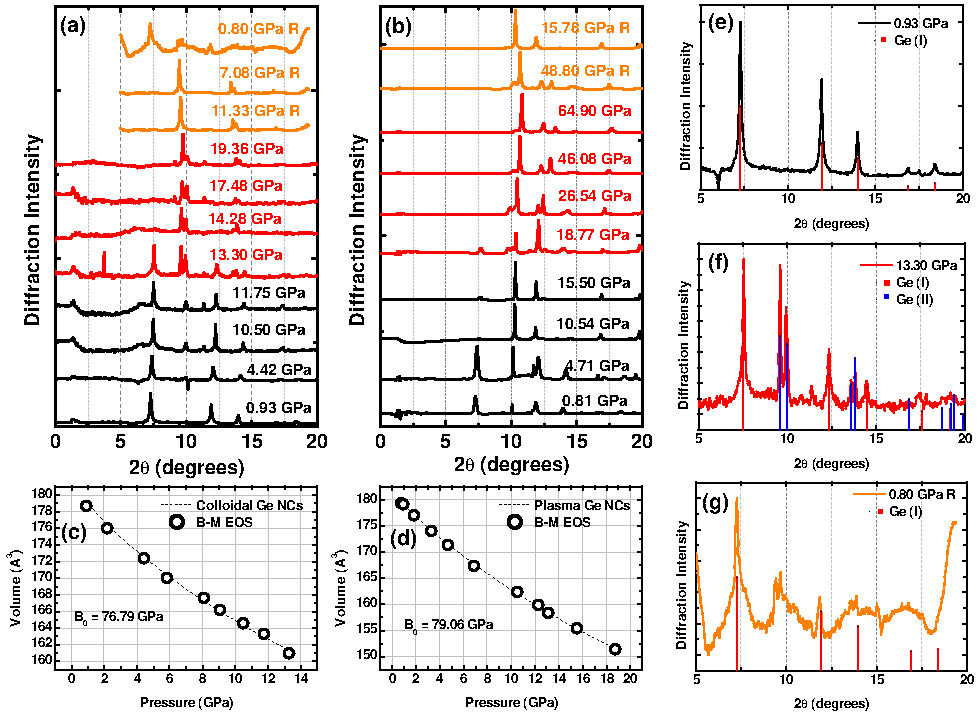
\includegraphics[width=\textwidth]{./chapter7/gepressure1.png}
\caption[Pressure-dependent XRD patterns for Ge NCs, phase analysis, and related XRD-derived structural data.]{(a) XRD patterns for 4 nm-diameter, colloidally synthesized Ge NCs at various indicated pressures.  Black curves indicate the presence of only the Ge(I) phase.  Red curves indicate the Ge(II) phase.  Orange curves indicate diffraction patterns acquired on pressurization downstrokes ("R") subsequent to pressurization to 19.36 GPa.  (b) XRD patterns for 4 nm-diameter, plasma synthesized Ge NCs at various applied pressures (indicated).  (c) XRD-derived unit cell volume as a function of pressure for colloidally synthesized NCs, along with a fit to the Burch-Murnaghan (B-M) equation of state and the resulting bulk modulus ($B_0$). (d) Same as (c), but for plasma-synthesized NCs. (e)-(g) Indicate XRD pattern for 4 nm-diameter, colloidally synthesized Ge NCs at (e) 0.93 GPa, with red vertical lines indicating the diffraction angles for the Ge(I) phase.  (f) 13.30 GPa, with red vertical lines indicating the diffraction angles for the Ge(I) phase and blue vertical lines indicating the diffraction angles for the Ge (II) phase.  (g) 0.80 GPa following pressurization to 19.36 GPa and subsequent depressurization to 0.80 GPa in roughly 5 GPa steps.  Red lines indicate diffraction angles for the Ge (I) phase.}
\label{f:gepressure1}
\end{center}
\end{figure}

Figure \ref{f:gepressure1} presents the experimental results of this XRD study of Ge NCs. Fig. \ref{f:gepressure1}(a) shows XRD patterns for the colloidally prepared Ge NCs referenced above, while Fig. \ref{f:gepressure1}(b) shows XRD patterns for the plasma-synthesized sample.  The colloidally prepared sample exhibits the Ge(I) (cubic, diamond) structure at ambient pressures. Diffraction peaks associated with the metallic Ge(II) ($\beta$-Sn) phase become apparent at $\sim$13 GPa, suggesting a phase transition which is elevated relative to bulk Ge \cite{PhysRevB.34.362}. Upon reversal of the pressure, the Ge NCs exhibit structural hysteresis, with Ge(II) peaks still present at a pressure of $\sim$7 GPa. Eventually, at 0.8 GPa, the Ge(I) phase is recovered. The plasma synthesized sample (Fig. \ref{f:gepressure1}(b)) exhibits similar behavior, but with a slightly elevated Ge(I) $\rightarrow$ Ge(II) phase transition pressure of 16.77 GPa. While experimental difficulties limited the maximum pressure of the colloidal Ge NC studies to 20 GPa, the plasma-synthesized NCs were pressurized to 70 GPa.  Upon depressurization, these samples also exhibit slight recovery of the Ge(I) phase. This is in contrast to Si, which exhibits complete and irreversible amorphization of the sample upon depressurization following a transition to the $\beta$-Sn phase. Figures \ref{f:gepressure1}(e), (f), (g) display a phase analysis of the XRD data, with vertical lines indicating the known diffraction peak positions for the Ge phases described here. \par
Figures \ref{f:gepressure1}(c) and (d) display unit cell volume for both Ge samples as a function of applied pressure, determined in the same fashion as for Si NCs and described above. Again, we fit these data to the third order Birch Murnaghan equation of state (Eq. \ref{eq:sipressure1}). The data are fit by Eq. \ref{eq:sipressure1} extremely well and yield bulk moduli of 76.79 GPa for the colloidal sample and 79.06 GPa for the plasma-synthesized sample. Both of these values are comparable to the 78 GPa bulk modulus reported for bulk Ge. A similar agreement between nanoscale and bulk phases is noted for Si above, but this agreement is in stark contrast to binary NC compositions. 

\section{Molecular Dynamics Simulations of Nanocrystal Pressurization}

To further explore the interesting structural behavior observed experimentally and presented above, we performed MD simulations of Si and Ge nanoparticles experiencing hydrostatic pressure applied by a pressure-transmitting medium. Our pressurization routine is the same used to derive the pressurized NC structures presented in chapter 5, which we elaborate on here. A faceted nanoparticle is first generated using experimentally known surface energies along with the Wulff construction. A box containing roughly 200,000 argon atoms (depending on NC size) is also created, and the Si NC placed in the center. Following this, any argon atoms having positions within 2\r{A} of a Si NC atom are deleted. Si-Si, Si-H, Ge-Ge, and Ge-H interactions are modeled according to the Tersoff potential \cite{PhysRevB.37.6991}. Interactions between the NC atoms (group-IV elements and H) and the fluid are modeled by a Lennard-Jones potential. Fluid-fluid interactions are modeled by a purely repulsive Lennard-Jones potential (i.e. cutoff set to $2\sigma^{1/6}$) to avoid freezing of the pressure-transmitting medium at high pressure. A timestep of 0.1 fs used to allow for accurate simulation of Si-H and Ge-H vibrations. After the initial geometry is created, the system is simulated for 2 ps in the NVE ensemble to allow fluid atoms to fill the space left by the deletion procedure described above. After that step, the system is simulated in the NPT ensemble (starting at 0 GPa) for a 15 ps equilibration run; this was determined to be sufficient to stabilize the pressure and temperature in the system. Following equilibration, a 5 ps production run was carried out. After production, the pressure is increased in steps of 0.25 GPa and the procedure repeated.

\subsection{The Impact of Surface Termination}

While utilizing MD simulations to explore the wurtzite-to-rocksalt phase transformation in CdSe nanocrystals, Gr{\"u}nwald and co-workers note the importance of including surface passivation due to its effect on NC surface energies \cite{grunwald2006mechanisms}. A number of studies have noted that pressure-induced phase transitions in CdSe begin with nucleation events on the NC surface \cite{grunwald2006mechanisms, grünwald2009nucleation, grunwald2009transition, grünwald2012metastability}. Because binary NCs can (and in practice often do) exhibit ion-rich surfaces, it is possible that that the elemental composition (rendering non-stoichiometric surfaces impossible) of group-IV NCs is responsible for the compressibility identical to that of the bulk phase. While the exact role played by the surface is a multifaceted issue, because surface ligands likely affect interactions with the solvent as well as the surface energies, we do note here that surface termination clearly affects NC response to applied hydrostatic pressure.

\begin{figure}
\begin{center}
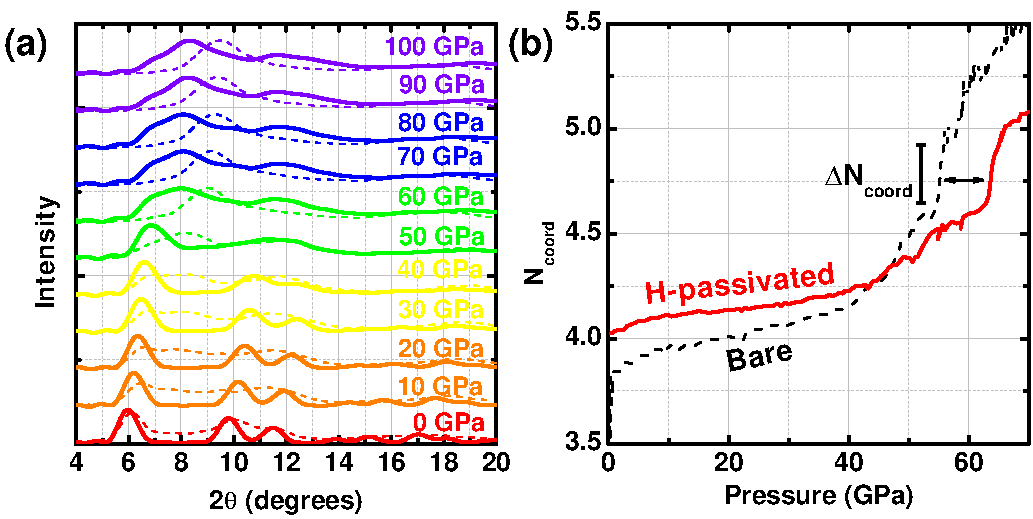
\includegraphics[width=\textwidth]{./chapter7/md1.png}
\caption[Comparison of simulated XRD and coordination number for bare and H-passivated Si NCs.]{(a) Simulated XRD patterns for a 2.4 nm-diameter Si NC at pressures spanning 0-100 GPa. Pressures are color-coded and indicated on the figure. Solid lines represent an H-passivated Si NC, while dashed lines represent a bare Si NC. (b) Average number of nearest numbers for each atom as a function of applied pressure for a bare (black, dashed lines) and passivated (red, solid lines) Si NC. $\Delta$N$_{\mathrm{coord}}$ indicates a discontinuity in the coordination number likely associated with a phase transition.}
\label{f:md1}
\end{center}
\end{figure}

Figure \ref{f:md1}(a) displays the simulated XRD diffraction pattern for a bare and H-terminated 2.4 nm-diameter Si NCs spanning pressures from 0-100 GPa. We calculate X-ray diffraction patterns by solving the Debye scattering equation:
\begin{equation}\label{eq:debye}
I(Q) = \sum_i\sum_j f_i f_j \frac{\sin{Q|\vec{r}_i - \vec{r}_j|}}{Q|\vec{r}_i - \vec{r}_j|}
\end{equation}
In Equation \ref{eq:debye}, $|\vec{r}_i - \vec{r}_j|$ is the distance between atoms $i$ and $j$, $f_i$ is the atomic scattering factor of atom $i$; this is an element-specific quantity which is wavelength-dependent and known in general, and $Q$ is scattering vector, related to the experimental X-ray wavelength $\lambda$ via $Q = |\vec{Q}| = 4\pi\sin{\theta/\lambda}$. In calculating the XRD patterns presented here we utilized the experimental X-ray energies (30 keV for Ge and 37 keV for Si). While the behavior exhibited by each nanocrystal is qualitatively similar, the structural evolution of the H-terminated NC seems to lag behind the bare NC. This is reflected in an analysis of the average coordination number presented by Si atoms in each simulation, shown in Fig. \ref{f:md1}(b). In particular, a phase transition, as evidenced by a discontinuity in the average coordination number seems to occur at $\sim$50 GPa for the bare NC, while a similar discontinuity is seen at $\sim$60 GPa for the H-passivated NC. While both of these pressures are considerably higher than the phase transition pressures observed experimentally, this is likely to the utilization of the Tersoff potential, which knowingly overestimates the absolute phase transition pressure but correctly captures trends and mechanisms in the bulk phase \cite{durandurdu2008diamond, PhysRevB.50.14952}. For the work presented in this chapter, we have studied H-passivated Si and Ge NCs; while these species are not an exact mimic of the alkyl termination experienced by the particles studied experimentally, the H-passivation scheme still presents a covalent surface bond while remaining computationally tractable.

\subsection{Comparison of Experimental and Simulated Structural Changes}

\begin{figure}
\begin{center}
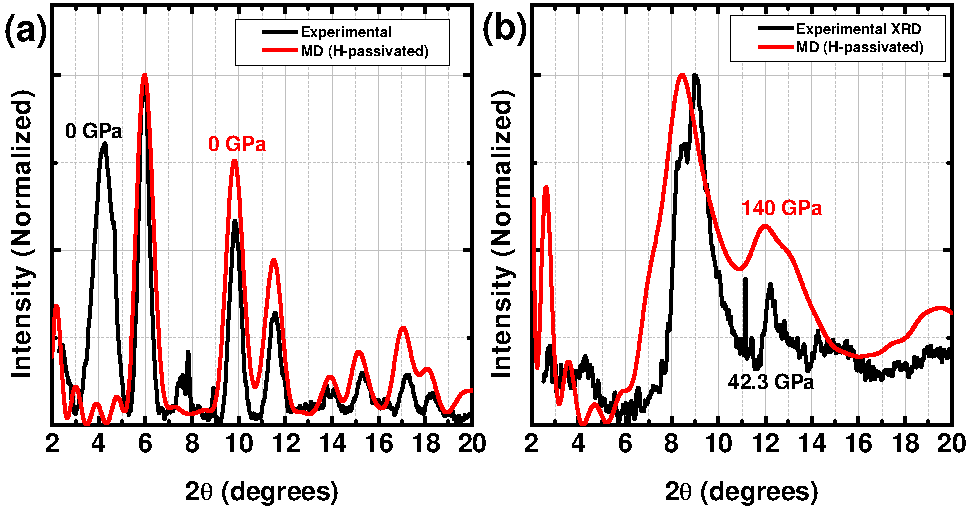
\includegraphics[width=\textwidth]{./chapter7/md2.png}
\caption[Comparison of simulated and experimental XRD patterns for passivated Si NCs.]{(a) Comparison of experimentally-observed (black) and MD derived (red) XRD patterns for Si NCs at ambient pressure. (b) Comparison of experimentally-observed (black) and MD derived (red) XRD patterns for Si NCs at pressures sufficient to induce a phase transition (140 GPa for MD, 42.3 GPa for experiment).}
\label{f:md2}
\end{center}
\end{figure}

Excepting the higher absolute pressure values needed to produce structural changes (likely related to the usage of a Tersoff interaction potential; see above), the computational pressurization scheme utilized here produces structures which agree well with those observed experimentally.  Figure \ref{f:md2} compares simulated and experimentally-observed XRD patterns for the low- and high-pressure phases of Si NCs. Fig. \ref{f:md2}(a) displays excellent agreement for the ambient-pressure structures, while \ref{f:md2}(b) also displays good agreement for the high-pressure phase. Note that while the pressure is much higher (140 GPa in the MD simulation compares reasonably well to an experimental pressure of 42.3 GPa), the peaks near 8$^{\circ}$ and 12.5$^{\circ}$ are associated with the $\beta$-Sn phase and are produced in both patterns. \par
We also note good agreement for Ge NCs. Figure \ref{f:md3}(a) displays a range of simulated XRD patterns for a 4 nm-diameter, H-passivated Ge nanocrystal at pressures spanning 0-100 GPa. The structure seems to undergo a large change between 50 and 60 GPa. Fig. \ref{f:md3}(b) compares the low- and high-pressure phases observed in our simulations to those observed experimentally (Fig. \ref{f:gepressure1}). Both phases show agreement, again with an elevated pressure (60 GPa) required to produce agreement with the experimental high-pressure phase (19 GPa). The peaks at 10$^{\circ}$ and 14$^{\circ}$ are characteristic of the $\beta$-Sn phase of Ge \cite{PhysRevB.34.362} and are present in both the simulated and experimental patterns. The agreement between experimentally-observed and simulation-derived XRD patterns suggests that the method of pressurization utilzied here is a suitable means of generating atomistic configurations of pressurized NCs.

\begin{figure}
\begin{center}
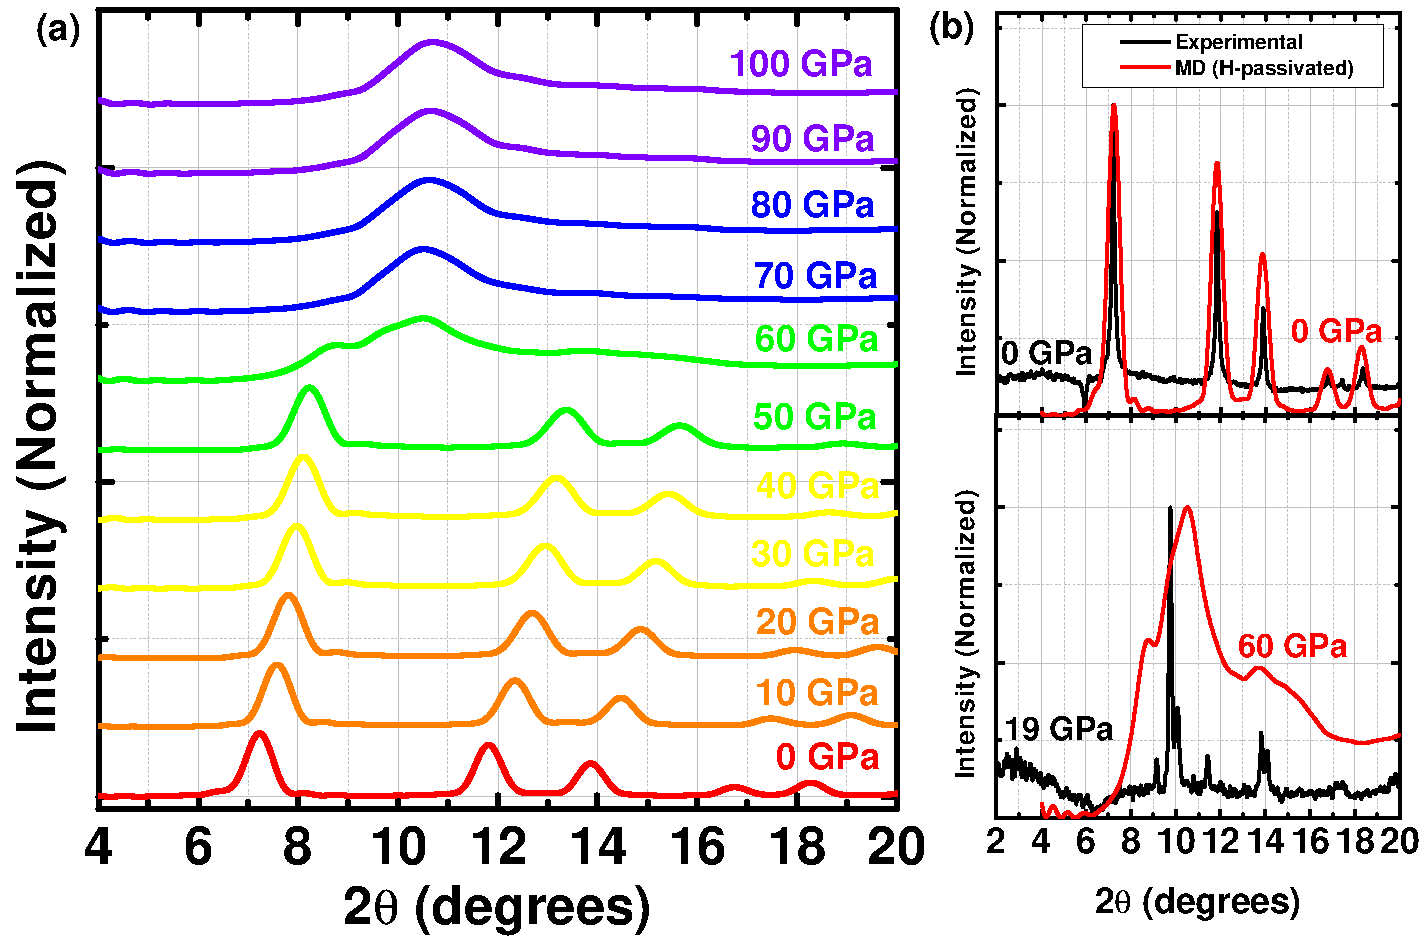
\includegraphics[width=\textwidth]{./chapter7/md3.png}
\caption[Simulated XRD patterns at a range of pressures and comparison of simulated and experimental XRD patterns for passivated Ge NCs.]{(a) Simulated XRD patterns for a 4 nm-diameter, H-passivated Ge NC at pressures spanning 0-100 GPa. Pressures are color-coded and indicated on the figure. (b) Top: Comparison of experimentally-observed (black) and MD derived (red) XRD patterns for Ge NCs at ambient pressure. Bottom: Comparison of experimentally-observed (black) and MD derived (red) XRD patterns for Ge NCs at pressures sufficient to induce a phase transition (60 GPa for MD, 19 GPa for experiment).}
\label{f:md3}
\end{center}
\end{figure}

\subsection{Analysis of Phase Transitions}

To obtain a quantitative measure of the local coordination environment of a given atom, we utilize an ordering parameter $q$,\cite{PhysRevB.28.784} which has been used previously to quantify nucleation events in supercooled liquid Si \cite{li2009nucleation}. We first compute the term $\bar{q}$, which is shown in Equation \ref{eq:md1}:
\begin{equation}\label{eq:md1}
\bar{q}_{lm}(i) = \frac{1}{N_b\left(i\right)}\sum_{j=1}^{N_b\left(i\right)} Y_{lm}\left(\theta\left(\vec{r}_{ij}\right), \phi\left(\vec{r}_{ij}\right)\right)
\end{equation}
In Eq. \ref{eq:md1}, $N_b(i)$ is the number of bonds for particle $i$, while $\theta$ and $\phi$ denote the azimuthal and polar angles of orientation for bond $\vec{r}_{ij}$. $Y_{lm}$ denote the spherical harmonics. From $\bar{q}_{lm}$, we may construct a $2l+1$ dimensional vector $\vec{q} = \left[\bar{q}_{l,-l}, \bar{q}_{l,-l+1}, ..., \bar{q}_{l, l-1}, \bar{q}_{l,l}\right]$ for each atom $i$ and compute:
\begin{equation}\label{eq:md2}
q_l = \frac{1}{N_b\left(i\right)}\sum_{j=1}^{N_b\left(i\right)}\frac{\vec{q}_l\left(i\right)\cdot\vec{q}_l\left(j\right)}{|\vec{q}_l\left(i\right)||\vec{q}_l\left(j\right)|}
\end{equation}

\begin{figure}
\begin{center}
\includegraphics[width=\textwidth]{./chapter7/md4.png}
\caption[Analysis of NC coordination environment using an ordering parameter and pressure-dependent crystal phase populations during MD simulations of pressurization.]{(a) and (b) display the distribution of local ordering parameter $q_4$ (Eq. \ref{eq:md2}) for Si and Ge NCs, respectively. In both (a) and (b), red bars represent the ambient-pressure histogram and blue bars represent the high-pressure histogram, with the pressures corresponding to each phase labeled on the figure. Both (a) and (b) also display a dashed line indicated the critical $q_4$ value, $q_c$, used to distinguish between phases. (c) and (d) display the number of atoms having either a diamond (red) or $\beta$-Sn environment (blue) as determined by the cutoff parameter $q_c$ for Si and Ge NCs, respectively.}
\label{f:md4}
\end{center}
\end{figure}

Figures \ref{f:md4}(a) and (b) show the distribution of of these local parameters using the fourth order spherical harmonics, which were found to produce the best discrimination between diamond and $\beta$-Sn phases. In order to quantify the local environment of atom $i$, a critical value $q_c$ is chosen such that atoms having $q_i < q_c$ are classified as one phase, while atoms having $q_i > q_c$ are classified as the other. For Si, atoms having $q_i < q_c$ are diamond phase, while the reverse is true for Ge (see Fig. \ref{f:md4}(a) and (b)). Using this criterion, the number of "diamond"-coordinated and the number of "$\beta$-Sn"-coordinated atoms was calculated along the range of pressures simulated. This is shown for a 2.4-nm diameter Si NC and a 4 nm-diameter Ge NC in Figure \ref{f:md4}(c) and (d) respectively. The diamond and $\beta$-Sn populations, for both NCs, show a rapid inflection and inversion around the the pressures indicated as phase transitions by XRD and nearest neighbor counting (see Figures \ref{f:md1} and \ref{f:md3}). This suggests that the choice of $q_c$ is suitable for analyzing the phase transition.\par

\begin{figure}
\begin{center}
\includegraphics[width=\textwidth]{./chapter7/md5.pdf}
\caption[Snapshots from MD simulations of NC pressurization color-coded according to ordering parameter analysis.]{Snapshots of NCs labeled according to composition and pressure. Each snapshot has atoms color coded according to coordination environment: Red for diamond, and blue for $\beta$-Sn, determined by the paramter $q_c$ as described in the main text. While pressure-transmitting fluid atoms and passivating H atoms are present in the simulation, they are not rendered in these snapshots.}
\label{f:md5}
\end{center}
\end{figure}

Figure \ref{f:md5} displays snapshots from the MD simulation trajectory for a Si and Ge NC. Atoms in Fig. \ref{f:md5} are colored according to their phase, determined as described above. Continuing the color scheme used in Fig. \ref{f:md4}, diamond atoms are colored red, while $\beta$-Sn atoms are colored blue. Both the Si and Ge particles display a noticeable but small contraction of the NC volume and a near-complete conversion to the $\beta$-Sn phase at high pressures. While both structures, and in particular the Ge NC, perhaps show a slight bias toward a surface-inward mechanism, it is not readily apparent from visual inspection of the trajectories alone what the spatial distribution of diamond- and $\beta$-Sn-coordinated atoms is along the trajectory.\par
The radial and pressure-dependent $q$ value for each Si (Ge) atom is plotted in Figure \ref{f:md6}(a)((b)). The Si NC shows little bias toward the surface.  While some atoms just beneath the surface quickly shift their coordination environment, the vast majority of atoms cross over the transition together, evident by the nearly-vertical front of $\beta$-Sn-coordinated atoms emerging at $P \approx 50$ GPa. The Ge NC, however, shows a significant fraction of surface atoms experiencing a $\beta$-Sn-like coordination environment at modest presssures prior to the major phase transition at $P \approx 60$ GPa, where a similar onset of $\beta$-Sn coordination appears. 

\begin{figure}
\begin{center}
\includegraphics[width=\textwidth]{./chapter7/md6.png}
\caption[Dependence of atomic coordination on radius and pressure during MD simulations of NC pressurization.]{(a) and (b) display the coordination environment (either diamond - red, or $\beta$-Sn - blue, determined by $q_c$ as described in the main text) as a function of pressure and NC radius for Si and Ge NCs, respectively. The sharp onset of $\beta$-Sn atoms at a particular pressure is indicative that a majority of NC atoms experience the phase transition together.}
\label{f:md6}
\end{center}
\end{figure}

\subsection{Results and Discussion}
It is worth noting that the results presented here are a preliminary study and are part of a larger work in progress. The size-dependence of the results will be especially important in determining the actual phase transition mechanism. While the Ge NC seems to exhibit the transition of surface atoms prior to core atoms, the Ge NC studied in this chapter is larger (4 nm-diameter) than the Si NC (2.4 nm-diameter). It is possible that 4 nm-diameter Si NCs may show a similar bias. Nevertheless, even the 4 nm-diameter Ge NC exhibits a simultaneous transition of a majority of atoms in the structure, and certainly to a greater extent than was observed in MD simulations of pressure-induced structural changes in CdSe NCs \cite{grünwald2012metastability}. This may suggest that the surface plays less of a role in initiating phase transitions in group-IV NCs than is the case for II-VI ionic NCs, and may explain the bulk-like compressibility of group-IV NCs noted here, as only a negligible fraction of atoms in bulk materials exist on surfaces. \par
Further work will be required to fully explore the origin of bulk-like compressibility in group-IV NCs and fully understand the mechanism of pressure-induced phase transitions in these materials. Firstly, while the Tersoff potential is known to overestimate the diamond $\rightarrow \beta$-Sn phase transition, there are also kinetic and statistical factors which are more appropriately treated by more advanced sampling methods. Because solid-solid transformations typically involve high kinetic barriers, phase transitions are statistically rare events under hydrostatic compression near the phase transition pressure \cite{grunwald2009transition, wittenberg2014real}. This typically requires observation timescales or size scales out of range of atomistic simulations. Instead, as we have done here, the usual solution is to simulate elevated pressures such that transformations readily occur on accessible timescales. Thus, it is possible that the mechansims observed here differ from those observed experimentally. A more rigorous analysis will necessarily utilize transition path sampling or forward-flux sampling algorithms capable of efficiently simulating statistically rare events \cite{grunwald2009transition, li2009nucleation}.

\section{Conclusions}
In this chapter we presented a characterization of pressure-induced structural changes in Si and Ge NCs. Colloidal dispersions of Si or Ge NCs were loaded into diamond anvil cells, pressurized, and examined using synchrotron-derived XRD. As has been observed for other NCs, Si and Ge nanocrystals exhibit elevated phase transition pressures relative to the bulk phase. In constrast to other NCs, however, both Si and Ge NCs exhibit a compressibility matching the bulk phase. To explore the origin of this behavior, we also carried out and presented here MD simulations of NC pressurization \emph{via} a pressure-transmitting fluid in a rough mimic of the actual diamond anvil cell experiment. Firstly, we noted good agreement between experimentally-observed and MD-derived XRD patterns, indicating the that use of a pressure-transmitting fluid is a suitable method for generating NC structures that resemble those generated during diamond anvil cell pressurization.\par
We also demonstrated that an ordering parameter based on spherical harmonics is capable of discriminating between low- (diamond) and high-pressure ($\beta$-Sn) phases in group-IV NCs. Using this ordering parameter, we found that a majority of NC atoms transition from $q < q_c$ to $q > q_c$ (that is, from diamond-like coordination to $\beta$-Sn-like coordination) collectively. This is somewhat in contrast to prior studies on CdSe NCs which suggest surface-led nucleation of the high-pressure phase. While we emphasize that more advanced MD trajectory sampling algorithms are necessary to confirm the phase transition mechanism explored here, our preliminary results suggest that group-IV NCs experience phase transitions in a more collective, rather than surface-dominated fashion. This may explain the bulklike compressibility of these NCs relative to binary NC compositions.
